\documentclass[a4paper,12pt, oneside, twocolumn]{scrartcl}
%\usepackage[ngerman]{babel}
\usepackage[utf8]{inputenc}
\setlength{\parindent}{0em}
\usepackage{eurosym}
\usepackage{amsmath}
\usepackage{amssymb}
\usepackage{dsfont}
\usepackage{polynom}
\usepackage{graphicx}
\usepackage{caption}
\usepackage{tikz}
\usepackage[a4paper,portrait,left=1.0cm,right=1.0cm,top=2cm,bottom=2cm]{geometry}
\usepackage{pgf} % Zur Einbindung der PGF Files
\usepackage{bm}

% Eigene Kommandos
\newcommand{\e}[1]{\text{e}^{#1}}
\newcommand{\rot}[2][rot]{\textcolor{#1}{#2}}
\newcommand{\gruen}[2][gruen]{\textcolor{#1}{#2}}
\newcommand{\frontcolor}[2][frontcolor]{\textcolor{#1}{#2}}
\newcommand{\gelb}[2][gelb]{\textcolor{#1}{#2}}
\newcommand{\orange}[2][orange]{\textcolor{#1}{#2}}
\newcommand{\blau}[2][blau]{\textcolor{#1}{#2}}
\newcommand{\hellblau}[2][hellblau]{\textcolor{#1}{#2}}
\newcommand{\lila}[2][lila]{\textcolor{#1}{#2}}
\newcommand{\dunkelrot}[2][dunkelrot]{\textcolor{#1}{#2}}
\newcommand{\dunkelgelb}[2][dunkelgelb]{\textcolor{#1}{#2}}

%%%%%%%%%%%%%%%%%%%%%%%%%%%%%%%%%%%%%%%%%%%%%%%%%%%%%%%%%%%%%%%%%%%%%%%
\newcommand{\norm}[1]{\left\lVert#1\right\lVert}
\newcommand{\dv}{\thinspace \mathrm{d}v}
\newcommand{\dw}{\thinspace \mathrm{d}w}
\newcommand{\dx}{\thinspace \mathrm{d}x}
\newcommand{\dy}{\thinspace \mathrm{d}y}
\newcommand{\dt}{\thinspace \mathrm{d}t}
\newcommand{\dr}{\thinspace \mathrm{d}r}
\newcommand{\ds}{\thinspace \mathrm{d}s}
\newcommand{\du}{\thinspace \mathrm{d}u}
\newcommand{\dz}{\thinspace \mathrm{d}z}
\newcommand{\dW}{\thinspace \mathrm{d}W}
\newcommand{\dX}{\thinspace \mathrm{d}X}
\newcommand{\dP}{\thinspace \mathrm{d}P}
\DeclareMathOperator*{\esssup}{ess\,sup}
\DeclareMathOperator*{\argmin}{arg\,min}

% Light Mode Customization
\usepackage{xcolor}
%\definecolor{backgroundgray}{RGB}{255,255,255}  % Weiß als Seitenhintergrund
\definecolor{textwhite}{RGB}{0,0,0}            % Schwarz als globale Schriftfarbe
\definecolor{boxgray}{RGB}{245,245,245}        % Sehr helles Grau für Box-Hintergründe
\definecolor{boxframe}{RGB}{200,200,200}       % Helles Grau für Box-Rahmen
\pagecolor{boxgray}  % Hintergrund auf Weiß
\color{textwhite}           % Text auf Schwarz

% Eigene Farben definiert (nun optimiert für hellen Hintergrund)
\definecolor{rot}{RGB}{204,0,0}
\definecolor{blau}{RGB}{0,102,204}
\definecolor{orange}{RGB}{204,85,0}
\definecolor{gruen}{RGB}{0,153,0}
\definecolor{dunkelgruen}{RGB}{0,153,0}
\definecolor{dunkelblau}{RGB}{0,128,128}
\definecolor{backcolor}{RGB}{235,245,255}
\definecolor{frontcolor}{RGB}{0,153,0}
\definecolor{hellblau}{RGB}{180,210,235}
\definecolor{lila}{RGB}{153,0,153}
\definecolor{gelb}{RGB}{204,153,0}
\definecolor{dunkelrot}{RGB}{153,0,51}
\definecolor{dunkelgelb}{RGB}{153,153,0}
\usepackage[backend=biber,style=numeric]{biblatex}
\addbibresource{references.bib}

% Ränder und Layout für geteilte Ansicht
\usepackage{multicol}
\setlength{\columnsep}{1cm}  % Abstand zwischen den Spalten

% Keine Seitenzahl
\pagestyle{empty}

% Begin des Dokuments
\begin{document}



\vspace{-1em} % Reduzierter Abstand

 % Zweispaltige Darstellung

\section*{Dynamics of Robots}
We use the principle of least action \cite{siciliano2010} with $L= T-V$ 
where $T$ is the kinetic energy and $V$ is the potential energy to get the Euler-Lagrange equations:
%
\begin{align*}
  \delta  \int L(t,\bm{q},\dot{\bm{q}}) \dt = 0 \Rightarrow  \frac{d}{dt} \frac{\partial T}{\partial \dot{\bm{q}}} - \frac{\partial T}{\partial \bm{q}} + \frac{\partial V}{\partial \bm{q}}  = 0
\end{align*}

For a rigid body system, we can express the kinetic energy $T$ as: \cite{spong2004}
%
\begin{align*}
    T = \frac{1}{2} \dot{\bm{q}}^T M(\bm{q}) \dot{\bm{q}} \text{with } M(\bm{q}) &\text{: Inertia matrix}
\end{align*}
%
We can compute the Inertia matrix $M(\bm{q})$ using the kinetic energy $T$ of the system:
%
\begin{align*}
    M(\textbf{q}) 
    &=
    \sum_{i=1}^n m_i J_{v_i}^T J_{v_i} + J_{\omega_i}^T I_i J_{\omega_i} 
    \quad
    J_v = \frac{\partial \textbf{r}}{\partial \textbf{q}} 
    \quad 
    J_\omega = \frac{\partial \boldsymbol{\omega}}{\partial \dot{\textbf{q}}}
\end{align*}
%
where $m_i$ is the mass of link $i$, $I_i$ is the inertia tensor of link $i$,
$J_{v_i}$ is the linear velocity Jacobian of link $i$, 
and $J_{\omega_i}$ is the angular velocity Jacobian of link $i$.
%
\subsection*{Two Link Revolute}
 We use the generalized coordinates 
 $\bm{q} = \begin{bmatrix} \gruen{\theta_1}, \rot{\theta_2} \end{bmatrix}$ 
for the two-link revolute manipulator.
%
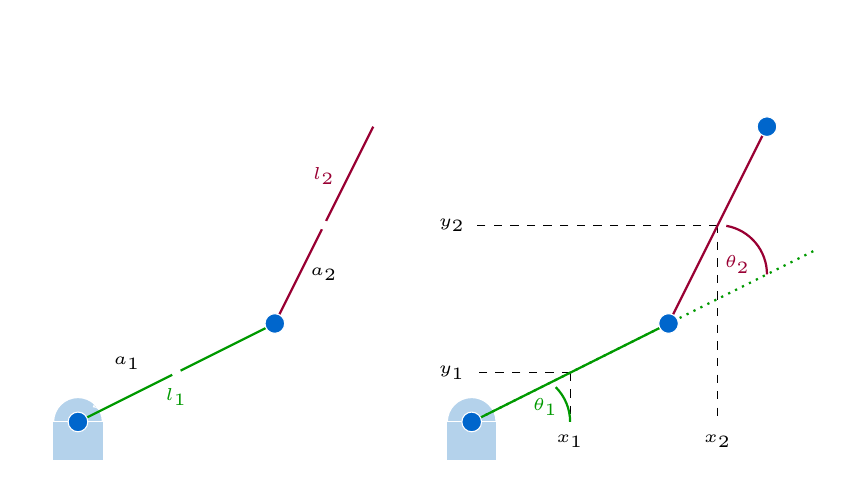
\begin{tikzpicture}[scale = 1.25, every node/.style={transform shape}]
    % Koordinatensystem
    %\draw[very thin, gray] (-5,-5) grid (5,5); % Raster
    %\draw[->] (-5,0) -- (5,0); % x-Achse
    %\draw[->] (0,-5) -- (0,5); % y-Achse
    
    % Achsen und Hilfslinien
    \draw[white, dashed, ->] (0.0,-1.0) -- (3.5,-1.0);
    \draw[white, dashed, ->] (0.0,-1.0) -- (0.0,3.0);
    
    % Schwerpunkte
    \draw[dashed] (1.0,-0.5) -- (1.0,-1.0);
    \draw[dashed] (1.0,-0.5) -- (0,-0.5);
    \node at (-0.2, -0.5) {\tiny $y_1$};  % Punktbeschriftung
    \node at (1, -1.2) {\tiny $x_1$}; 
    \draw[dashed] (2.5,1) -- (0.0,1);
    \draw[dashed] (2.5,1) -- (2.5,-1);
    \node at (-0.2, 1.0) {\tiny $y_2$};  % Punktbeschriftung
    \node at (2.5, -1.2) {\tiny $x_2$}; 

    % Erste Zeichnung (Original)
    \fill[hellblau] (-4,-1) circle (0.25);  % Füllt das Objekt mit hellblau
    \draw[white, line width = 0.2mm] (-4,-1) circle (0.25);  % Weißer Rand um das Objekt
    
    \draw[white, line width = 0.2mm] (-4.25,-1.4) rectangle (-3.75,-1);  % Weißer Rand um das Rechteck
    \fill[hellblau] (-4.25,-1.4) rectangle (-3.75,-1);  % Füllt das Rechteck mit hellblau
    \draw[thick, white] (-4.5,-1.4) -- (-3.5,-1.4);
    
    % Grüne Linie angepasst (Endpunkt auf (-2.0, 0.0))
    \draw[thick, gruen] (-4,-1) -- (-2.0,0.0);
    
    % Rote Linie angepasst (von (-2.0, 0.0) nach (-1.0, 2.0))
    \draw[thick, dunkelrot] (-2.0,0.0) -- (-1.0,2.0);
    
    % Glieder
    \fill[blau] (-2.0,0.0) circle (0.1);
    \draw[white, thin] (-2.0,0.0) circle (0.1);  % Weißer Rand um das Objekt
    \fill[blau] (-4.0,-1.0) circle (0.1);
    \draw[white, thin] (-4.0,-1.0) circle (0.1);  % Weißer Rand um das Objekt
    
	% Beschriftungen
	\node at (-3, -0.75) {\tiny $\gruen{l_1}$};  % 
	\node at (-1.5, 1.5) {\tiny $\dunkelrot{l_2}$};  % 
	
	% Schwerpunkte 
	\fill[white] (-3.0,-0.5) circle (0.05);
	\fill[white] (-1.5,1) circle (0.05);
	
	\draw[white, <->] (-1.85,0.15) -- (-1.5,0.85);
	\draw[white, <->] (-3.85,-0.85) -- (-3.1,-0.45);
	
	% Beschriftungen
	\node at (-3.5, -0.4) {\tiny $a_1$};  % 
	\node at (-1.5, 0.5) {\tiny $a_2$};  % 
    
    % Zweite Zeichnung (verschoben um 4 Einheiten entlang der x-Achse)
    \fill[hellblau] (0,-1) circle (0.25);  % Füllt das Objekt mit hellblau
    \draw[white, line width = 0.2mm] (0,-1) circle (0.25);  % Weißer Rand um das Objekt
    
    \draw[white, line width = 0.2mm] (-0.25,-1.4) rectangle (0.25,-1);  % Weißer Rand um das Rechteck
    \fill[hellblau] (-0.25,-1.4) rectangle (0.25,-1);  % Füllt das Rechteck mit hellblau
    \draw[thick, white] (-0.5,-1.4) -- (0.5,-1.4);
    
    % Grüne Linie (verschoben)
    \draw[thick, gruen] (0,-1) -- (2.0,0.0);
    \draw[thick, gruen, dotted] (0,-1) -- (3.5,0.75);
    
    % Rote Linie (verschoben)
    \draw[thick, dunkelrot] (2.0,0.0) -- (3.0,2.0);
    
    % Glieder
    \fill[blau] (2.0,0.0) circle (0.1);
    \draw[white, thin] (2.0,0.0) circle (0.1);  % Weißer Rand um das Objekt
    \fill[blau] (0.0,-1.0) circle (0.1);
    \draw[white, thin] (0.0,-1.0) circle (0.1);  % Weißer Rand um das Objekt
    \fill[blau] (3.0,2.0) circle (0.1);
    \draw[white, thin] (3.0,2.0) circle (0.1);  % Weißer Rand um das Objekt
    
    % Winkel
    \draw [gruen, thick] (1,-1)  arc[start angle=0,end angle=45,radius=0.5cm];
	\node at (0.75, -0.85) {\tiny $\gruen{\theta_1}$};  % Winkelbeschriftung
	
	\draw [dunkelrot, thick] (3,0.5)  arc[start angle=0,end angle=80,radius=0.5cm];
	\node at (2.7, 0.6) {\tiny $\dunkelrot{\theta_2}$};  % Winkelbeschriftung
\end{tikzpicture}

By using the coordinates of the centers of mass, 
%
{\small
\begin{align*}
    \bm{r}_1
    =
    \begin{pmatrix}
        a_1 \cdot \cos(\gruen{\theta_1}) \\
        a_1 \cdot \sin(\gruen{\theta_1}) \\
        0
    \end{pmatrix}
    \;
    \bm{r}_2
    =
    \begin{pmatrix}
        l_1 \cdot \cos(\gruen{\theta_1}) 
        + a_2 \cos(\gruen{\theta_1} + \dunkelrot{\theta_2}) \\
        l_1 \cdot \sin(\gruen{\theta_1}) 
        + a_2 \sin(\gruen{\theta_1} + \dunkelrot{\theta_2}) \\
        0
    \end{pmatrix}
\end{align*}
}
we can derive the Jacobians $J_{v_i}$ and $J_{\omega_i}$ and thus the inertia matrix $M(\bm{q})$.
Plugging $M(\bm{q})$ into the Euler-Lagrange equations,
we have the following equations of motion for a robotic manipulator:
%
\begin{align*}
    M(\bm{q}) \ddot{\bm{q}} &+ C(\bm{q}, \dot{\bm{q}}) \dot{\bm{q}} + G(\bm{q}) = \bm{\tau} \\
    C(\bm{q}, \dot{\bm{q}}) &\text{: Coriolis and centrifugal matrix} \\
    G(\bm{q}) &\text{: Gravity vector} \\
    \bm{u} &\text{: Joint torques}
\end{align*}
\subsection*{Gripper extension}
We can model the gripper as an additional point mass $m_G$ at the end of the second link or 
as an additional third link with length $l_3$ and mass $m_3$.

    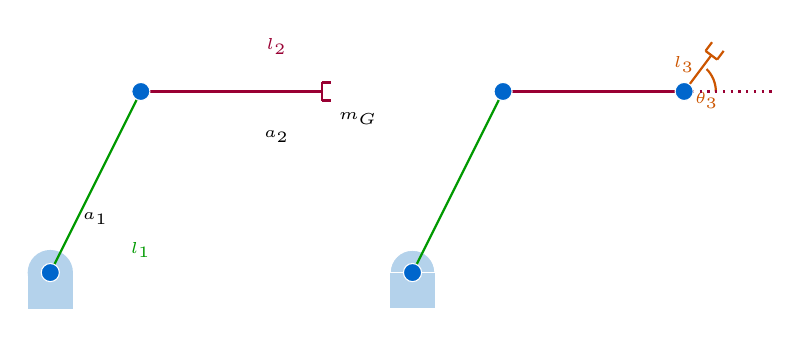
\begin{tikzpicture}[scale = 1.15, every node/.style={transform shape}]
        % Koordinatensystem
        %\draw[very thin, gray] (-5,-5) grid (5,5); % Raster
        %\draw[->] (-5,0) -- (5,0); % x-Achse
        %\draw[->] (0,-5) -- (0,5); % y-Achse
        
        % Erste Zeichnung (Original)
        \fill[hellblau] (-4,-1) circle (0.25);  % Füllt das Objekt mit hellblau
        %\draw[white, line width = 0.2mm] (-4,-1) circle (0.25);  % Weißer Rand um das Objekt
        
        %\draw[white, line width = 0.2mm] (-4.25,-1.4) rectangle (-3.75,-1);  % Weißer Rand um das Rechteck
        \fill[hellblau] (-4.25,-1.4) rectangle (-3.75,-1);  % Füllt das Rechteck mit hellblau
        %\draw[thick, white] (-4.5,-1.4) -- (-3.5,-1.4);
        
        % Grüne Linie angepasst (Endpunkt auf (-2.0, 0.0))
        \draw[thick, gruen] (-4,-1) -- (-3.0,1.0);
        
        % Rote Linie angepasst (von (-2.0, 0.0) nach (-1.0, 2.0))
        \draw[thick, dunkelrot] (-3.0,1.0) -- (-1.0,1.0);
        
        % Glieder
        \fill[blau] (-3.0,1.0) circle (0.1);
        \draw[white, thin] (-3.0,1.0) circle (0.1);  % Weißer Rand um das Objekt
        \fill[blau] (-4.0,-1.0) circle (0.1);
        \draw[white, thin] (-4.0,-1.0) circle (0.1);  % Weißer Rand um das Objekt
        
        % Beschriftungen
        \node at (-3, -0.75) {\tiny $\gruen{l_1}$};  % 
        \node at (-1.5, 1.5) {\tiny $\dunkelrot{l_2}$};  % 
        
        % Schwerpunkte 
        %\fill[white] (-3.0,-0.5) circle (0.05);
        %\fill[white] (-1.5,1) circle (0.05);
        
        %\draw[white, <->] (-1.85,0.15) -- (-1.5,0.85);
        %\draw[white, <->] (-3.85,-0.85) -- (-3.1,-0.45);
        
        % Beschriftungen
        \node at (-3.5, -0.4) {\tiny $a_1$};  % 
        \node at (-1.5, 0.5) {\tiny $a_2$};  % 

        \draw[dunkelrot, thick] (-1.0,0.9) -- (-1.0, 1.1);
        \draw[dunkelrot, thick] (-1.0,0.9) -- ++(0.1,0.0);
        \draw[dunkelrot, thick] (-1.0,1.1) -- ++(0.1,0.0);
        \node at (-0.6,0.7) {\tiny $m_G$}; % Beschriftung

        % Erste Zeichnung (Original) verschoben um +4 in x
        \fill[hellblau] (0,-1) circle (0.25);  % Füllt das Objekt mit hellblau
        \draw[white, line width = 0.2mm] (0,-1) circle (0.25);  % Weißer Rand um das Objekt
        
        \draw[white, line width = 0.2mm] (-0.25,-1.4) rectangle (0.25,-1);  % Weißer Rand um das Rechteck
        \fill[hellblau] (-0.25,-1.4) rectangle (0.25,-1);  % Füllt das Rechteck mit hellblau
        \draw[thick, white] (-0.5,-1.4) -- (0.5,-1.4);
        
        % Grüne Linie angepasst (Endpunkt auf (1.0, 1.0))
        \draw[thick, gruen] (0,-1) -- (1.0,1.0);
        
        % Rote Linie angepasst (von (1.0, 1.0) nach (3.0, 1.0))
        \draw[thick, dunkelrot] (1.0,1.0) -- (3.0,1.0);

        % Orange Linie zum Greifobjekt
        \draw[thick, orange] (3.0,1.0) -- (3.3,1.4);
        \draw[thick, orange] (3.364,1.352) -- (3.236,1.448);
        \draw[thick, orange] (3.364,1.352) -- ++(0.072,0.096);
        \draw[thick, orange] (3.236,1.448) -- ++(0.072,0.096);

        % Winkel
        \draw [orange, thick] (3.35,1.0)  arc[start angle=0,end angle=45,radius=0.35cm];
	    \node at (3.25, 0.9) {\tiny $\orange{\theta_3}$};  % Winkelbeschriftung
        \draw[thick, dunkelrot, dotted] (3,1) -- (4.0,1.0);
        \node at (3.0, 1.3) {\tiny $\orange{l_3}$};

        \fill[blau] (3.0,1.0) circle (0.1);
        \draw[white, thin] (3.0,1.0) circle (0.1);  % Weißer Rand um das Objekt

        % Glieder
        \fill[blau] (1.0,1.0) circle (0.1);
        \draw[white, thin] (1.0,1.0) circle (0.1);  % Weißer Rand um das Objekt
        \fill[blau] (0.0,-1.0) circle (0.1);
        \draw[white, thin] (0.0,-1.0) circle (0.1);  % Weißer Rand um das Objekt
    \end{tikzpicture}

The second formulation requires the addition of a third generalized coordinate
$\orange{\theta_3}$, which represents the angle of the gripper relative to the second link.
The new generalized coordinates are
$\bm{q} = \begin{bmatrix} \gruen{\theta_1}, \dunkelrot{\theta_2}, \orange{\theta_3} \end{bmatrix}$.
The inertia matrix $M(\bm{q})$ must be recalculated to account for the additional link.

%
\section*{Foundations of Control Theory}

Our formulation of an optimal control problem is based on the procedure outlined in \cite{gerdts2012}.
Let $[t_0,t_f]$ be a fixed time interval,
    \begin{align*}
        \Phi &: \mathbb{R}^{n_{\bm{x}}} \to \mathbb{R}, \\
        L &: [t_0,t_f] \times \mathbb{R}^{n_{\bm{x}}}  \to \mathbb{R},  \\
        f &: [t_0,t_f] \times \mathbb{R}^{n_{\bm{x}}} \times \mathbb{R}^{n_{\bm{u}}} 
        \to \mathbb{R}^{n_{\bm{x}}}
    \end{align*}
    %
    sufficient smooth functions and $\mathcal{U} \subset \mathbb{R}^{n_{\bm{u}}}$ 
    a closed convex non-empty set. 
    %
    \begin{align*}
        \min_{\bm{u}} \int_{t_0}^{t_f} L(t,\bm{x}(t),\bm{u}(t)) \dt + \Phi(\bm{x}(t_f))
    \end{align*}
    %
    with respect to $\bm{x} \in W_{1,\infty}^{n_{\bm{x}}}([t_0,t_f]), 
    \bm{u} \in L_{\infty}^{n_{\bm{u}}}([t_0,t_f])$ and subject to
    %
    \begin{align*}
        \dot{\bm{x}}(t) = f(t,\bm{x}(t),\bm{u}(t)), \; \bm{x}(t_0) = \bm{x}_0, \; \bm{u}(t) \in \mathcal{U} 
    \end{align*}
    %\text{a.e. } t \in [t_0,t_f]

The necessary conditions for optimality 
are given by minimimum principle (see \cite{gerdts2012}):
%
\begin{align*}
    \dot{\bm{p}} = -H_{\bm{x}} \; \bm{p}(t_f) = \Phi_{\bm{x}}(\bm{x}(t_f)) \\
    H(t,\bm{x},\bm{u},\bm{p}) = L(t,\bm{x},\bm{u}) + \bm{p}^T f(t,\bm{x},\bm{u}) \\
    \bm{u}^* = \argmin_{\bm{u} \in \mathcal{U}} H(t,\bm{x}^*,\bm{u},\bm{p}^*)
\end{align*}

\section*{Linearisation Method}
Let 
$\textbf{x} = 
\begin{bmatrix}
    \textbf{q} \\
    \dot{\textbf{q}}
\end{bmatrix}$ we use the state space 
representation of the manipulator dynamics (compare \cite{ICIIECS2017}).
%
\begin{align*}
        \underbrace{
            \begin{bmatrix}
                \dot{\textbf{q}} \\ \ddot{\textbf{q}}
            \end{bmatrix}
    }_{
        \dot{\textbf{x}}
    }
    =
        \underbrace{
        \begin{bmatrix}
            \dot{\textbf{q}} \\
            M^{-1}(\textbf{q}) 
            \left[ 
                \bm{u} - C(\textbf{q}, \dot{\textbf{q}}) \dot{\textbf{q}} - G(\textbf{q}) 
                \right]
        \end{bmatrix}
    }_{
        f(\textbf{x}, \bm{u})
    }
\end{align*}

We linearize the system around an operating point:
%
\begin{align*}
    \dot{\bm{x}} 
    &= f(\bm{x},\bm{u}) \\
    &\approx \underbrace{f(\bm{x}^*,\bm{u}^*)}_{= 0} + 
    \underbrace{\frac{\partial f}{\partial x}(\bm{x}^*,\bm{u}^*)}_{A(\bm{x}^*,\bm{u}^*)}(\bm{x}-\bm{x}^*) 
    + \underbrace{\frac{\partial f}{\partial u}(\bm{x}^*,\bm{u}^*)}_{B(\bm{x}^*,\bm{u}^*)}(\bm{u}-\bm{u}^*) 
    \\
    &= A(\bm{x}^*,\bm{u}^*) \bar{\bm{x}} + B(\bm{x}^*,\bm{u}^*) \bar{\bm{u}}
\end{align*}

We get the equivalent linear system:
%
\begin{align*}
    \bar{\bm{x}}(t) = A \bar{\bm{x}}(t) + B \bar{\bm{u}}(t) 
    \; 
    \bar{\bm{x}} = \bm{0} \Leftrightarrow \bm{x} = \bm{x}^* 
\end{align*}

By assuming $f(\bm{x}^*,\bm{u}^*) = \bm{0}$ 
we get $\ddot{\bm{q}^*} = \dot{\bm{q}^*} = \bm{0}$. Thus we 
have the following derivates for our specific two link manipulator:
%
\begin{align*}
    A &=
        \begin{bmatrix}
        \bm{0} & I \\
        M^{-1}(\bm{q}^*) 
        \left[
            -\frac{\partial G}{\partial \bm{q}}(\bm{q}^*) 
        \right]
        & 
        \bm{0}
    \end{bmatrix}   
    \;
    B =
        \begin{bmatrix}
            \bm{0} \\
            M^{-1}(\bm{q}^*)
        \end{bmatrix}
\end{align*}

\subsection*{Solving using LQR}
We can solve the nonlinar optimal control problem
%
\begin{align*}
    \min_u & \int_0^\infty 
            (\bm{q} - \bm{q}_f)^T Q (\bm{q} - \bm{q}_f) 
            + (\bm{u} - \bm{u}_f)^T R (\bm{u} - \bm{u}_f) \dt \\
            	\textsf{s.t. } & M(\bm{q}) \ddot{\bm{q}} 
                + C(\bm{q},\dot{\bm{q}}) \dot{\bm{q}} 
                + G(\bm{q}) = \bm{u};
                \quad
                \bm{u}_f - G(\bm{q}_f) = \bm{0} 
\end{align*}
by solving the linearized problem using LQR:
%
\begin{align*}
    \min_{\bar{\bm{u}}} & \int_0^\infty 
            \bar{\bm{x}}^T Q \bar{\bm{x}} + \bar{\bm{u}}^T R \bar{\bm{u}} \dt 
            \quad\dot{\bar{\bm{x}}} = A \bar{\bm{x}} + B \bar{\bm{u}};
\end{align*}
with $\bar{\bm{x}} = \bm{x} - \bm{x}_f$ and $\bar{\bm{u}} = \bm{u} - \bm{u}_f$. 
The solution $K$ of the Riccati equation:
%
\begin{align*}
    Q - K B R^{-1} B^T K + KA + A^T K = 0 
\end{align*} 
%
gives us the optimal feedback law: 
%
\begin{align*}
    \bm{u}_i &= G(\bm{q}_f) - R^{-1} B^T K (\bm{x}_i - \bm{x}_f) \\
    \bm{x}_{i+1} &= \bm{x}_i + h \cdot f(\bm{x}_i, \bm{u}_i)  
\end{align*}

\section*{Gradient Methods}
We can also solve the optimal control problem 
%
\begin{align*}
    \min_{\bm{u}} &\int_{t_0}^{t_f} (\bm{u} - \bm{u}_f)^T \cdot R \cdot (\bm{u} - \bm{u}_f) \dt + \Phi(\bm{x}(t_f)) \\
    \Phi(\bm{x}(t_f)) &= (\bm{q}(t_f) - \bm{q}_f)^T \cdot Q \cdot (\bm{q}(t_f) - \bm{q}_f) \\
    \dot{\bm{x}} = f(\bm{x},\bm{u}) 
    &=  
    \begin{bmatrix}
        \dot{\bm{q}} \\
        M^{-1}(\bm{q}) \cdot ( - C(\bm{q},\dot{\bm{q}}) \cdot \dot{\bm{q}} - G(\bm{q}) + \bm{u} )
    \end{bmatrix}
\end{align*}
%
The adjoint equation is given by:
\begin{align*}
    \dot{\bm{p}} 
    =
    -
    \frac{\partial f}{\partial \bm{x}}^T \cdot \bm{p},
    \quad
    \bm{p}(t_f) 
    = \begin{bmatrix}
        2 Q (\bm{q}(t_f) - \bm{q}_f) \\
        \bm{0}
    \end{bmatrix}
\end{align*}
%
The gradient of the Hamiltonian is given by:
%
\begin{align*}
    \nabla J(\bm{u})
    =
    2 R \cdot (\bm{u} - \bm{u}_f) +     
    \begin{bmatrix}
        \bm{0}_2 \\
        M^{-1}(\bm{q})
    \end{bmatrix} \cdot 
    \begin{bmatrix}
        \bm{p}_{\bm{q}} \\
        \bm{p}_{\dot{\bm{q}}}
    \end{bmatrix}
\end{align*}

{\small
\begin{itemize}
    \item[1)] Forward integration of the state equation
    %
    \begin{align*}
        \bm{x}_{i+1} = \bm{x}_i + h \cdot f(\bm{x}_i, \bm{u}_i) \Rightarrow \bm{X} = \{\bm{x}_0, \ldots, \bm{x}_N\}
    \end{align*}
    %
    \item[2)] Backward integration of the adjoint equation
    %
    \begin{align*}
        \bm{p}_N 
        &= 
        \begin{bmatrix}
            2 Q (\bm{q}(t_f) - \bm{q}_f) \\
            \bm{0}
        \end{bmatrix} 
        \bm{p}_{i-1} 
        = \bm{p}_{i} + h  \cdot
        \begin{bmatrix}
           \bm{0}_2 & I_2 \\
            \frac{\partial \ddot{\bm{q}}}{\partial \bm{q}}
           &
           \frac{\partial \ddot{\bm{q}}}{\partial \dot{\bm{q}}}
        \end{bmatrix}
        \cdot \bm{p}_{i}
    \end{align*}
    %
    using finite differences to compute 
    %
    \begin{align*}
        \bm{x}_{\pm}  &= \bm{x} \pm \epsilon \cdot \bm{e}_j \; 
        \frac{\partial \ddot{\bm{q}}}{\partial x_j}
        \approx
        \frac{\ddot{\bm{q}}(\bm{x}_{+}) - \ddot{\bm{q}}(\bm{x}_{-})}{2 \epsilon}
        \Rightarrow 
        \bm{P} = \{\bm{p}_0, \ldots, \bm{p}_N\}
    \end{align*}
    %
    \item[3)] Gradient descent for $i = 0, \ldots, N-1$:
    %
    \begin{align*}
        \bm{u}_{i+1} &= \bm{u}_i - \alpha_j \cdot 
        \left[
            2 R \cdot (\bm{u}_i - \bm{u}_f) + M^{-1}(\bm{q}_i) \cdot \bm{P}_{\dot{\bm{q}},i}
        \right]  
    \end{align*}
    by using the armijo rule to $\alpha_j$.
\end{itemize}
}


\small
\printbibliography

\end{document}